A nikon Z bajonettcsatlakozás a Nikon tükör nélküli kameráin (MILC) használt objektívcsatlakozás. A csatlakoztatott eszköz és a fényképezőgépváz közti kommunikáció teljes mértékben elktronikusan történik. Itt minimum annyi információ átvitel zajlik, mint a Nikon F bajonett esetében, így az összes F bajonettes kiegészítő irányításához szükséges adatot a Z bajonettes fényképezőgép képes elküldeni és fogadni. A rögzítés az F csatlakozásnál használt módszerekkel történik, azonban dimenzióiban és implementációjában különbözik. "A rendszer nagy objektív foglalata egy 55mm-es belső átmérővel és egy rövid, 16mm-es foglalat-filmsík távolsággal van ellátva (...)."\cite{Nikon_Z}
%The system’s large lens mount features a 55mm inner diameter and short 16mm flange focal distance

\begin{figure}[H]
	\centering
	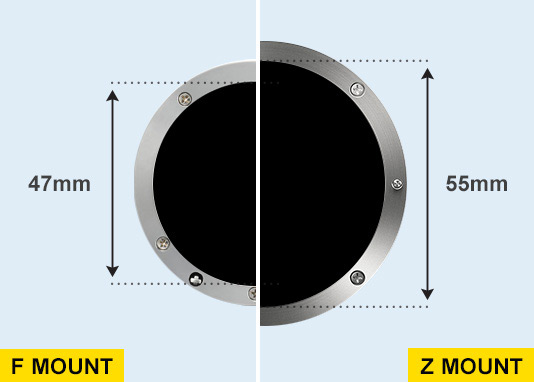
\includegraphics[width=0.5\linewidth]{img/F-mount-vs-Z-mount-illustration.jpg}
    \cite{Nikon_Z}
	\caption{Nikon F (bal) és Nikon Z (bal) objektívfoglalatok belső átmérője közti különbség}
	\label{fig:F_vs_Z_meret}
\end{figure}